\documentclass[11pt, spanish]{article}
\usepackage[spanish]{babel}
\selectlanguage{spanish}
\usepackage[utf8]{inputenc}
\usepackage{amsmath}
\usepackage{amsfonts}
\usepackage{amsthm}
\usepackage{float}
\usepackage{graphicx}
\pdfminorversion=5 
\pdfcompresslevel=9
\pdfobjcompresslevel=2

% Margenes
\usepackage[left=2cm,right=2cm,top=2cm,bottom=2cm]{geometry}
%Espaciado
%\linespread{1.3}


\title{Introducción al Procesamiento Digital de Imágenes - Práctica 4 (bis)}
\date{}
\author{Gonzalo Ciruelos Rodríguez (LU: 63/14)}

\begin{document}
\maketitle

Para preparar el entorno para poder ejecutar todos los programas,
primero debe tenerse instalado \texttt{python3} (y su \texttt{pip} correspondiente).
Luego, debe ejecutarse 
\begin{verbatim}
    virtualenv -p python3 venv 
    . venv/bin/activate
    pip install -r requirements.txt 
\end{verbatim}

\noindent para instalar las dependencias (pillow (para imágenes), numpy y matplotlib).



\section{Ejercicio 1}

Transformadas de Fourier graficadas.

Modo de uso
\begin{verbatim}
    python3 practica4/ej1.py
\end{verbatim}

\subsection{Transformada de Fourier de dimensión 8 en 1D}

\[
\begin{bmatrix}
e^{\frac{-2 \pi i \cdot 0 \cdot 0}{8}} & e^{\frac{-2 \pi i \cdot 0 \cdot 1}{8}} & e^{\frac{-2 \pi i \cdot0 \cdot 2}{8}}
& e^{\frac{-2 \pi i \cdot 0 \cdot 3}{8}} & e^{\frac{-2 \pi i \cdot 0 \cdot 4}{8}} & e^{\frac{-2 \pi i \cdot 0 \cdot
5}{8}} & e^{\frac{-2 \pi i \cdot 0 \cdot 6}{8}} & e^{\frac{-2 \pi i \cdot 0 \cdot 7}{8}} \\
e^{\frac{-2 \pi i \cdot 1 \cdot 0}{8}} & e^{\frac{-2 \pi i \cdot 1 \cdot 1}{8}} & e^{\frac{-2 \pi i \cdot1 \cdot 2}{8}}
& e^{\frac{-2 \pi i \cdot 1 \cdot 3}{8}} & e^{\frac{-2 \pi i \cdot 1 \cdot 4}{8}} & e^{\frac{-2 \pi i \cdot 1 \cdot
5}{8}} & e^{\frac{-2 \pi i \cdot 1 \cdot 6}{8}} & e^{\frac{-2 \pi i \cdot 1 \cdot 7}{8}} \\
e^{\frac{-2 \pi i \cdot 2 \cdot 0}{8}} & e^{\frac{-2 \pi i \cdot 2 \cdot 1}{8}} & e^{\frac{-2 \pi i \cdot2 \cdot 2}{8}}
& e^{\frac{-2 \pi i \cdot 2 \cdot 3}{8}} & e^{\frac{-2 \pi i \cdot 2 \cdot 4}{8}} & e^{\frac{-2 \pi i \cdot 2 \cdot
5}{8}} & e^{\frac{-2 \pi i \cdot 2 \cdot 6}{8}} & e^{\frac{-2 \pi i \cdot 2 \cdot 7}{8}} \\
e^{\frac{-2 \pi i \cdot 3 \cdot 0}{8}} & e^{\frac{-2 \pi i \cdot 3 \cdot 1}{8}} & e^{\frac{-2 \pi i \cdot3 \cdot 2}{8}}
& e^{\frac{-2 \pi i \cdot 3 \cdot 3}{8}} & e^{\frac{-2 \pi i \cdot 3 \cdot 4}{8}} & e^{\frac{-2 \pi i \cdot 3 \cdot
5}{8}} & e^{\frac{-2 \pi i \cdot 3 \cdot 6}{8}} & e^{\frac{-2 \pi i \cdot 3 \cdot 7}{8}} \\
e^{\frac{-2 \pi i \cdot 4 \cdot 0}{8}} & e^{\frac{-2 \pi i \cdot 4 \cdot 1}{8}} & e^{\frac{-2 \pi i \cdot4 \cdot 2}{8}}
& e^{\frac{-2 \pi i \cdot 4 \cdot 3}{8}} & e^{\frac{-2 \pi i \cdot 4 \cdot 4}{8}} & e^{\frac{-2 \pi i \cdot 4 \cdot
5}{8}} & e^{\frac{-2 \pi i \cdot 4 \cdot 6}{8}} & e^{\frac{-2 \pi i \cdot 4 \cdot 7}{8}} \\
e^{\frac{-2 \pi i \cdot 5 \cdot 0}{8}} & e^{\frac{-2 \pi i \cdot 5 \cdot 1}{8}} & e^{\frac{-2 \pi i \cdot5 \cdot 2}{8}}
& e^{\frac{-2 \pi i \cdot 5 \cdot 3}{8}} & e^{\frac{-2 \pi i \cdot 5 \cdot 4}{8}} & e^{\frac{-2 \pi i \cdot 5 \cdot
5}{8}} & e^{\frac{-2 \pi i \cdot 5 \cdot 6}{8}} & e^{\frac{-2 \pi i \cdot 5 \cdot 7}{8}} \\
e^{\frac{-2 \pi i \cdot 6 \cdot 0}{8}} & e^{\frac{-2 \pi i \cdot 6 \cdot 1}{8}} & e^{\frac{-2 \pi i \cdot6 \cdot 2}{8}}
& e^{\frac{-2 \pi i \cdot 6 \cdot 3}{8}} & e^{\frac{-2 \pi i \cdot 6 \cdot 4}{8}} & e^{\frac{-2 \pi i \cdot 6 \cdot
5}{8}} & e^{\frac{-2 \pi i \cdot 6 \cdot 6}{8}} & e^{\frac{-2 \pi i \cdot 6 \cdot 7}{8}} \\
e^{\frac{-2 \pi i \cdot 7 \cdot 0}{8}} & e^{\frac{-2 \pi i \cdot 7 \cdot 1}{8}} & e^{\frac{-2 \pi i \cdot7 \cdot 2}{8}}
& e^{\frac{-2 \pi i \cdot 7 \cdot 3}{8}} & e^{\frac{-2 \pi i \cdot 7 \cdot 4}{8}} & e^{\frac{-2 \pi i \cdot 7 \cdot
5}{8}} & e^{\frac{-2 \pi i \cdot 7 \cdot 6}{8}} & e^{\frac{-2 \pi i \cdot 7 \cdot 7}{8}} \\
\end{bmatrix}
\]
\[=
\begin{bmatrix}
1 & 1 & 1 & 1 & 1 & 1 & 1 & 1 \\
1 & e^{\frac{-1}{4} \pi i} & e^{\frac{-1}{2} \pi i} & e^{\frac{-3}{4} \pi i} & e^{-1 \pi i} & e^{\frac{-1}{4} \pi i} &
e^{\frac{-1}{2} \pi i} & e^{\frac{-3}{4} \pi i} \\
1 & e^{\frac{-1}{2} \pi i} & e^{-1 \pi i} & e^{\frac{-1}{2} \pi i} & e^{-2 \pi i} & e^{\frac{-1}{2} \pi i} & e^{-3 \pi
i} & e^{\frac{-1}{2} \pi i} \\
1 & e^{\frac{-3}{4} \pi i} & e^{\frac{-1}{2} \pi i} & e^{\frac{-1}{4} \pi i} & e^{-3 \pi i} & e^{\frac{-3}{4} \pi i} &
e^{\frac{-1}{2} \pi i} & e^{\frac{-1}{4} \pi i} \\
1 & e^{-1 \pi i} & e^{-2 \pi i} & e^{-3 \pi i} & e^{-4 \pi i} & e^{-5 \pi i} & e^{-6 \pi i} & e^{-7 \pi i} \\
1 & e^{\frac{-1}{4} \pi i} & e^{\frac{-1}{2} \pi i} & e^{\frac{-3}{4} \pi i} & e^{-5 \pi i} & e^{\frac{-1}{4} \pi i} &
e^{\frac{-1}{2} \pi i} & e^{\frac{-3}{4} \pi i} \\
1 & e^{\frac{-1}{2} \pi i} & e^{-3 \pi i} & e^{\frac{-1}{2} \pi i} & e^{-6 \pi i} & e^{\frac{-1}{2} \pi i} & e^{-9 \pi
i} & e^{\frac{-1}{2} \pi i} \\
1 & e^{\frac{-3}{4} \pi i} & e^{\frac{-1}{2} \pi i} & e^{\frac{-1}{4} \pi i} & e^{-7 \pi i} & e^{\frac{-3}{4} \pi i} &
e^{\frac{-1}{2} \pi i} & e^{\frac{-1}{4} \pi i} \\
\end{bmatrix}
\]

\begin{figure}[H]
\centering
  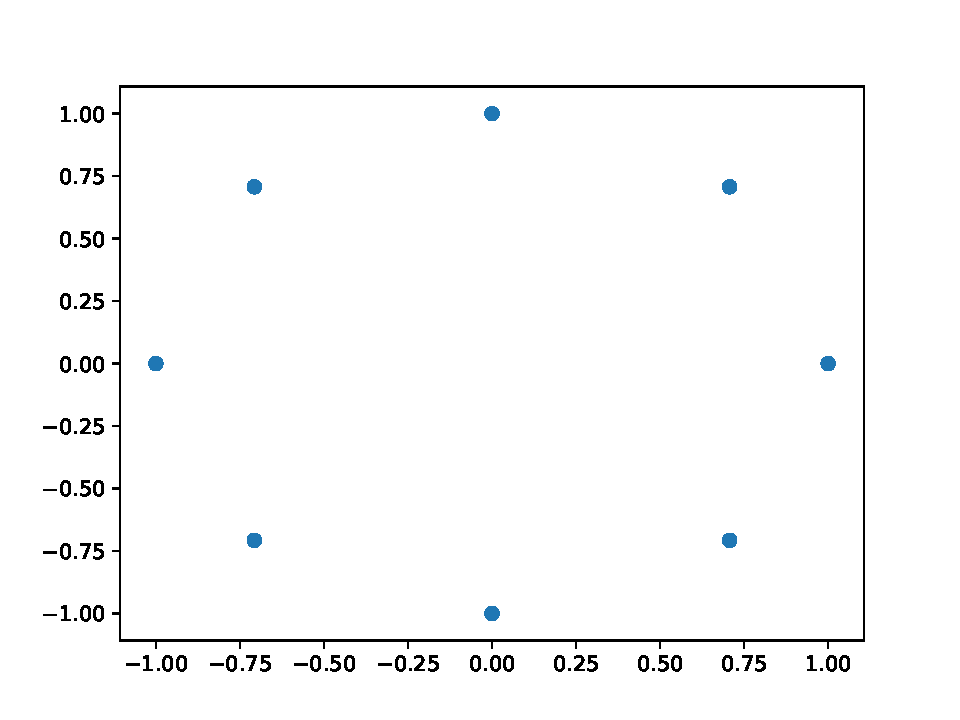
\includegraphics[height=6cm]{informe-imgs/ej1.pdf}
  \caption{\texttt{python3 practica4/ej1.py}}
\end{figure}

\subsection{Transformada de Fourier de dimensión 8 en 2D}

La matriz es de $8\times 8\times 8\times 8$, pero los puntos en el plano complejo son los mismos:

\begin{figure}[H]
\centering
  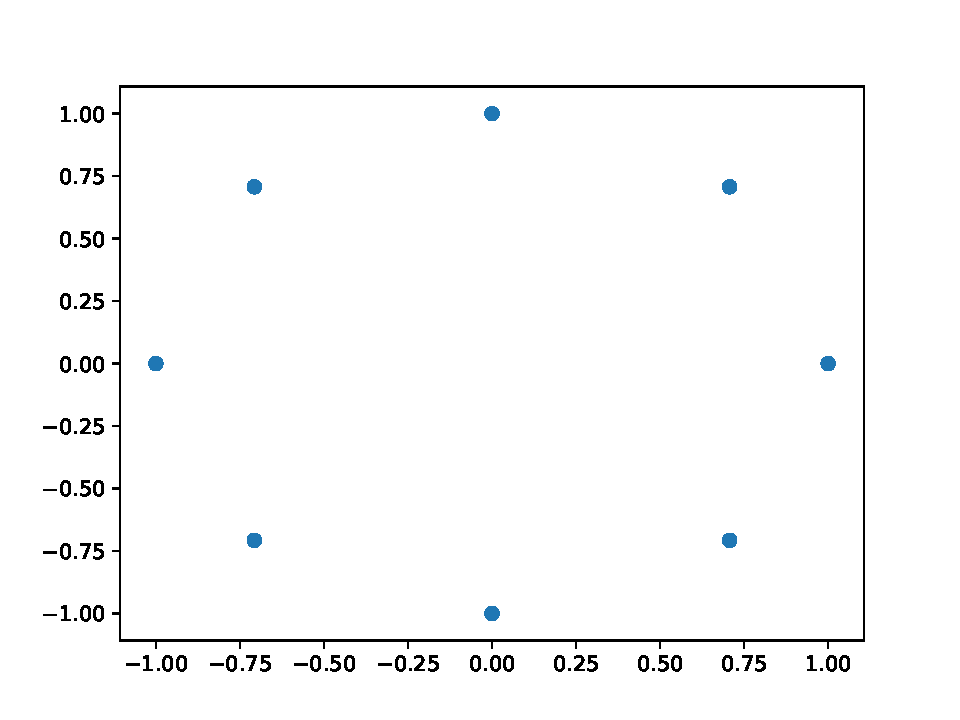
\includegraphics[height=6cm]{informe-imgs/ej1.pdf}
  \caption{\texttt{python3 practica4/ej1.py}}
\end{figure}

\newpage
\section{Ejercicio 2}
Modo de uso
\begin{verbatim}
    python3 practica4/ej2.py
\end{verbatim}

Supongamos que lo hacemos con la señal propuesta, o sea $x = [1, 1, 1, 1, 1, 1, 1, 1, 1, 0, 0, 0, 0, 0, 0, 0]$.

\begin{figure}[H]
\centering
  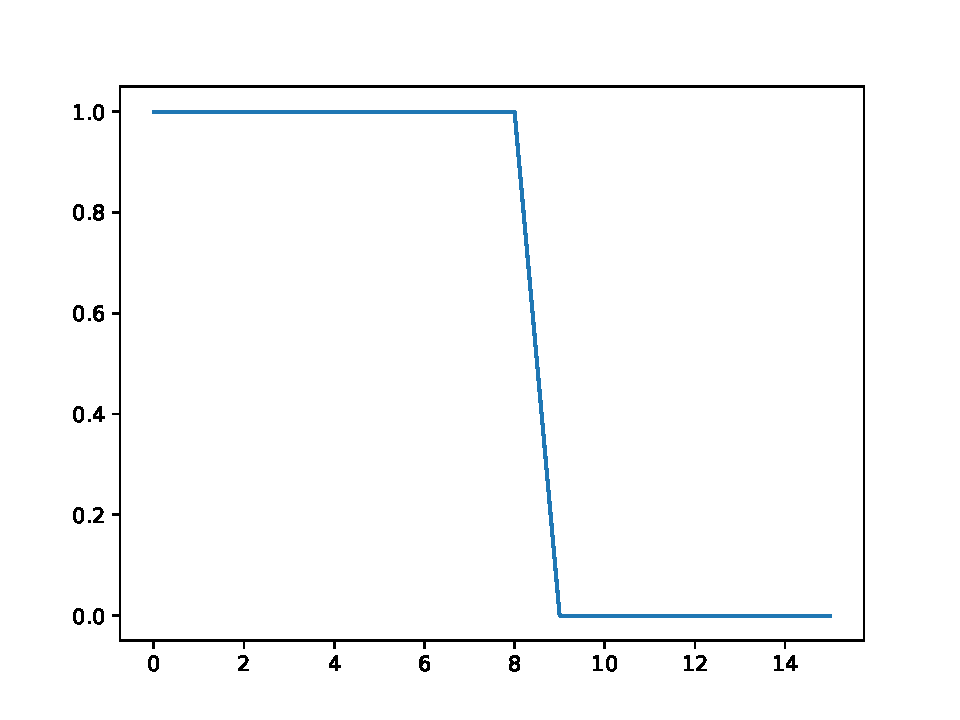
\includegraphics[height=6cm]{informe-imgs/ej2-senial.pdf}
  \caption{La señal}
\end{figure}

\subsection{Suprimiendo las frecuencias altas}

Notar que en el pasaje de la segunda señal a la tercera señal, las frecuencias más altas desaparecen.

Este es en realidad un filtro pasa bajo, con lo cual, tal como se ve, su efecto es el de suavizar un poco la señal.
\begin{figure}[H]
\centering
  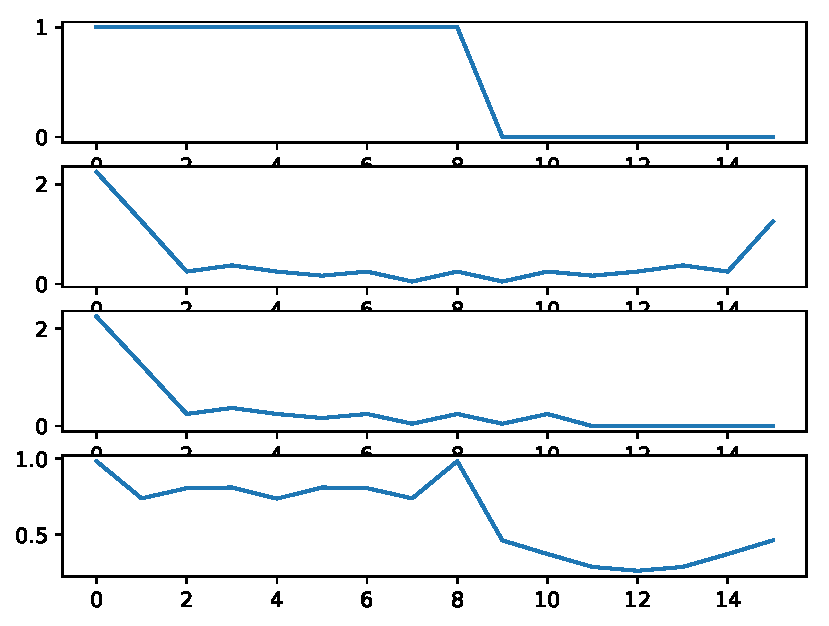
\includegraphics[height=6cm]{informe-imgs/ej2-elimino-alto.pdf}
  \caption{Filtro elimino alto. Señal original, DFT, DFT post-filtro, IDFT.}
\end{figure}

\subsection{Suprimiendo las frecuencias bajas}

Notar que en el pasaje de la segunda señal a la tercera señal, las frecuencias más bajas desaparecen.

Este es en realidad un filtro pasa alto, con lo cual el resultado es el realce de los bordes: notar que las frecuencias
más fuertes son aquellas donde la señal original tenía picos (el principio y el señal cuentan como picos pues es
periódica.

\begin{figure}[H]
\centering
  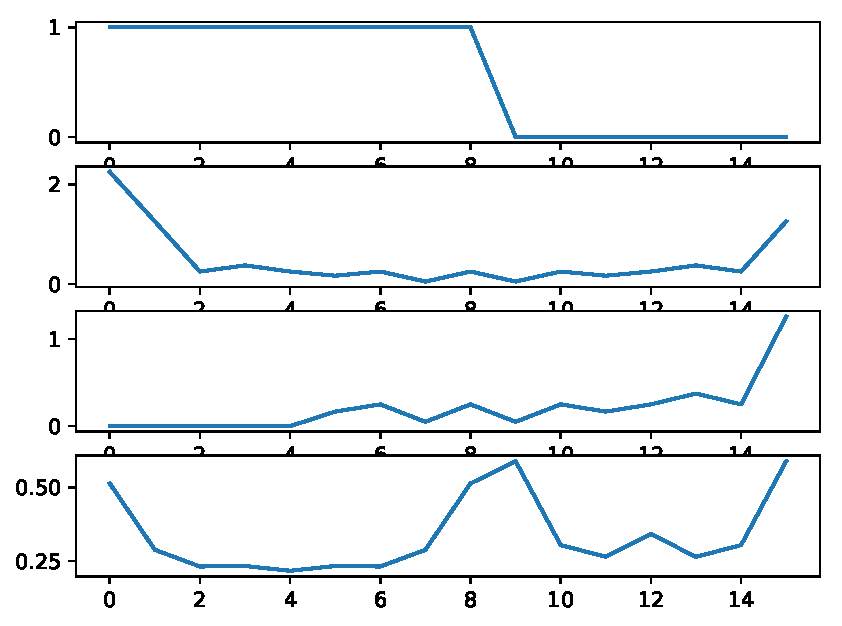
\includegraphics[height=6cm]{informe-imgs/ej2-elimino-bajo.pdf}
  \caption{Filtro elimino bajo. Señal original, DFT, DFT post-filtro, IDFT.}
\end{figure}

\subsection{Suprimiendo las frecuencias medias}

Notar que en el pasaje de la segunda señal a la tercera señal, las frecuencias del medio desaparecen.
Esto no cambia mucho la señal, pues las frecuencias intermedias ya eran bastante bajas.
\begin{figure}[H]
\centering
  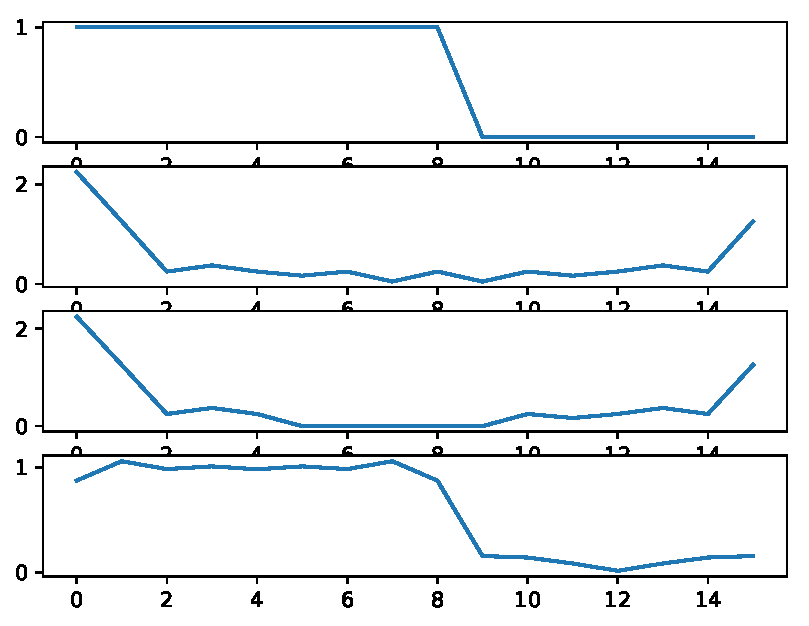
\includegraphics[height=6cm]{informe-imgs/ej2-elimino-medio.pdf}
  \caption{Filtro elimino medio. Señal original, DFT, DFT post-filtro, IDFT.}
\end{figure}

\newpage
\section{Ejercicio 3}

Este ejercicio se basa en hacer la DFT y la IDFT de cada imagen propuesta. Omitimos la IDFT porque da igual que la
imagen original.
Para cada imagen, mostramos esa imagen, el módulo de la transformada de fourier y la fase.

Modo de uso
\begin{verbatim}
    python3 practica4/fourier.py <img>
\end{verbatim}

Por ejemplo, para la imagen de Lena el resultado sería este:

\begin{figure}[H]
\centering
  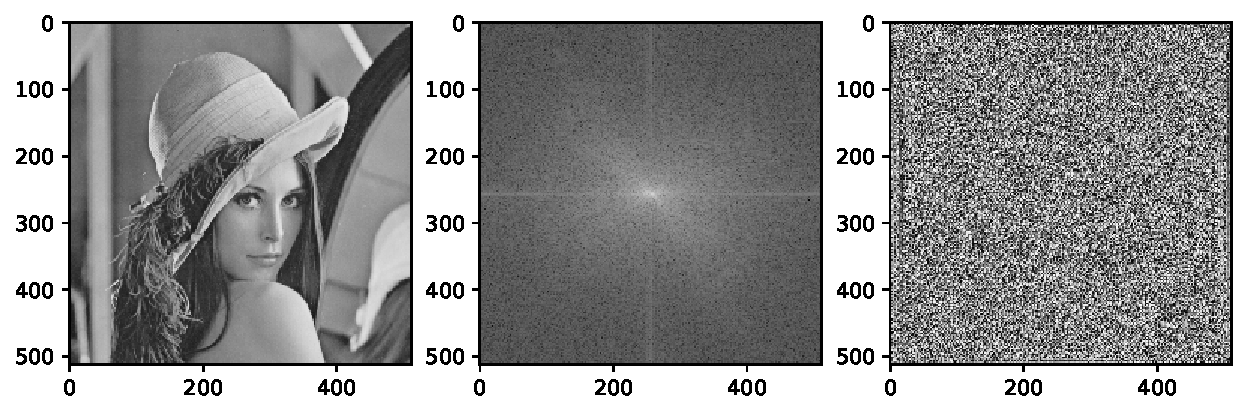
\includegraphics[height=6cm]{informe-imgs/ej3-lena.pdf}
  \caption{\texttt{python practica4/fourier.py lena.png}}
\end{figure}

\subsection{a) un cuadrado central}
Primero tenemos el cuadrado central.
\begin{figure}[H]
\centering
  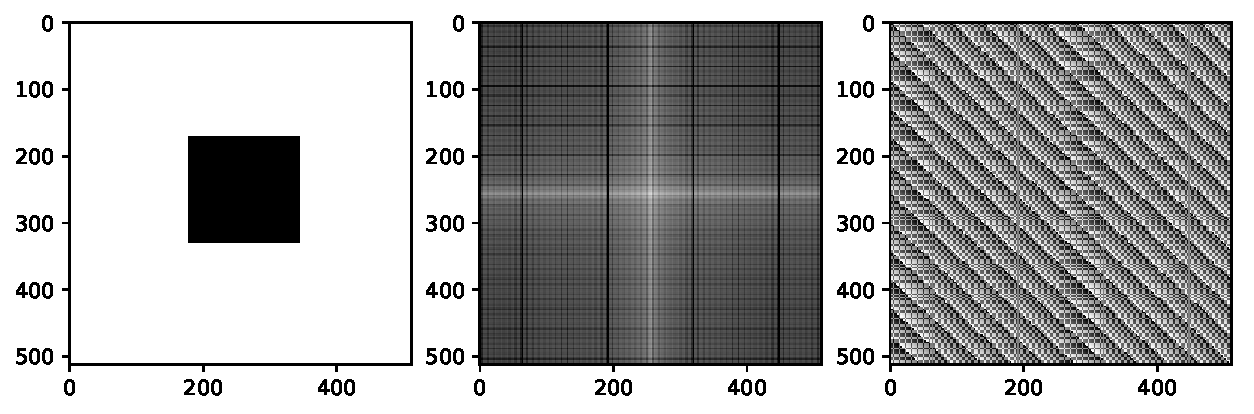
\includegraphics[height=6cm]{informe-imgs/ej3-a.pdf}
  \caption{\texttt{python practica4/fourier.py imgs-ej3/img-a.png}}
\end{figure}

\subsection{b) un cuadrado transladado}

Luego tenemos el cuadrado transladado. Notar que tiene sentido que el módulo haya dado igual en la imágen anterior que
en esta, pues como consideramos señales ``periódicas'' entonces las señales son las mismas.
\begin{figure}[H]
\centering
  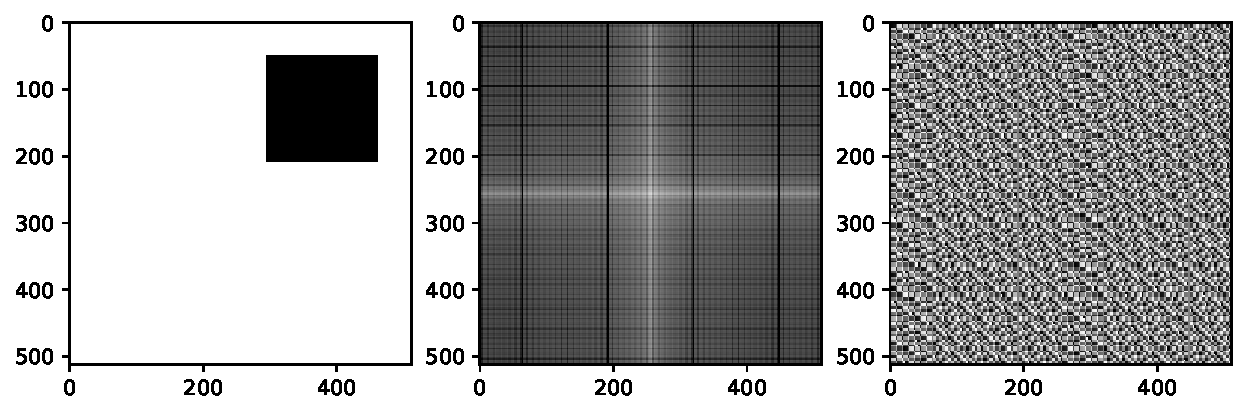
\includegraphics[height=6cm]{informe-imgs/ej3-b.pdf}
  \caption{\texttt{python practica4/fourier.py imgs-ej3/img-b.png}}
\end{figure}

\subsection{c) un rectángulo}
\begin{figure}[H]
\centering
  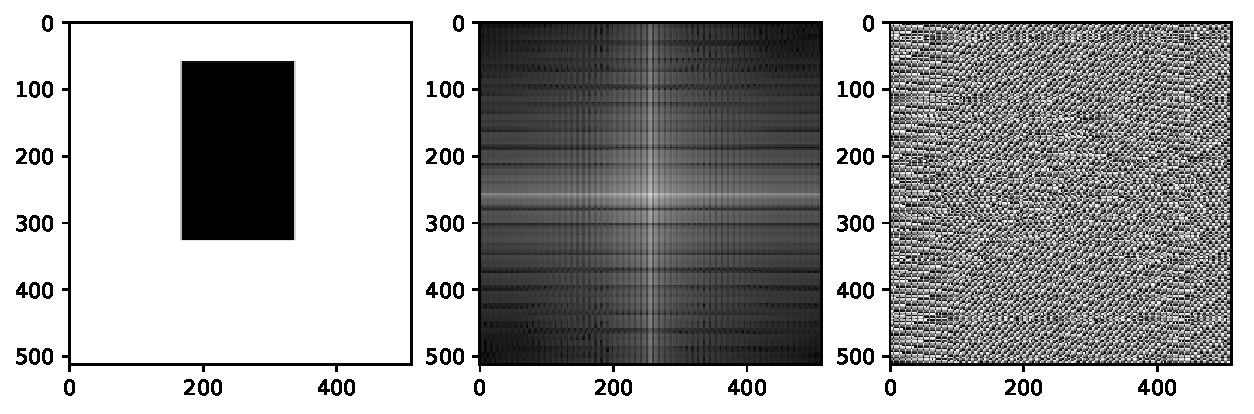
\includegraphics[height=6cm]{informe-imgs/ej3-c.pdf}
  \caption{\texttt{python practica4/fourier.py imgs-ej3/img-c.png}}
\end{figure}

\subsection{d) dos rectángulos de diferente tamaño}
\begin{figure}[H]
\centering
  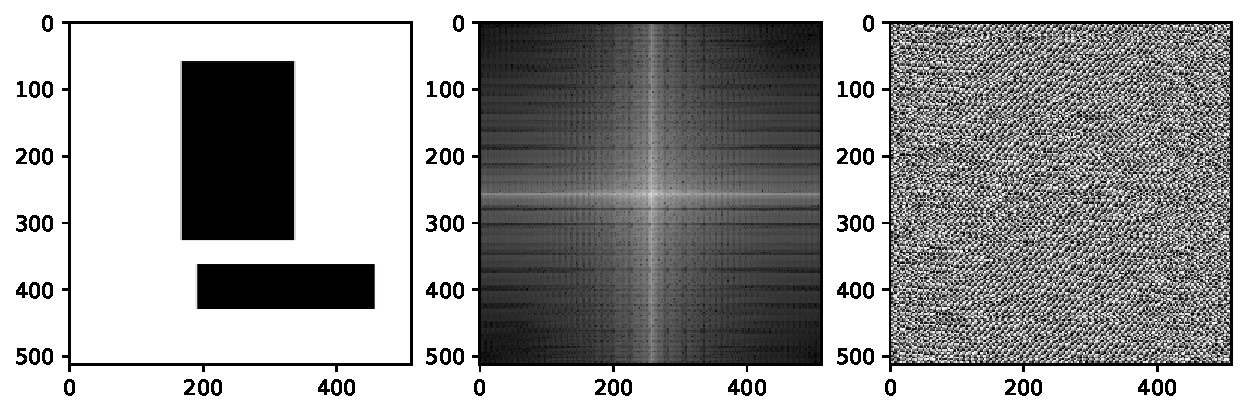
\includegraphics[height=6cm]{informe-imgs/ej3-d.pdf}
  \caption{\texttt{python practica4/fourier.py imgs-ej3/img-d.png}}
\end{figure}

\subsection{e) una línea vertical}
Notar que en las imágenes de la línea vertical, la fase está orientada de la misma manera que la linea.

Además, el gráfico del módulo es una tiene una linea dominante perpendicular a la linea original. Esto se debe a que las
frecuencias dominantes de la señal original son exactamente aquellas perpendiculares a la línea recta original.
\begin{figure}[H]
\centering
  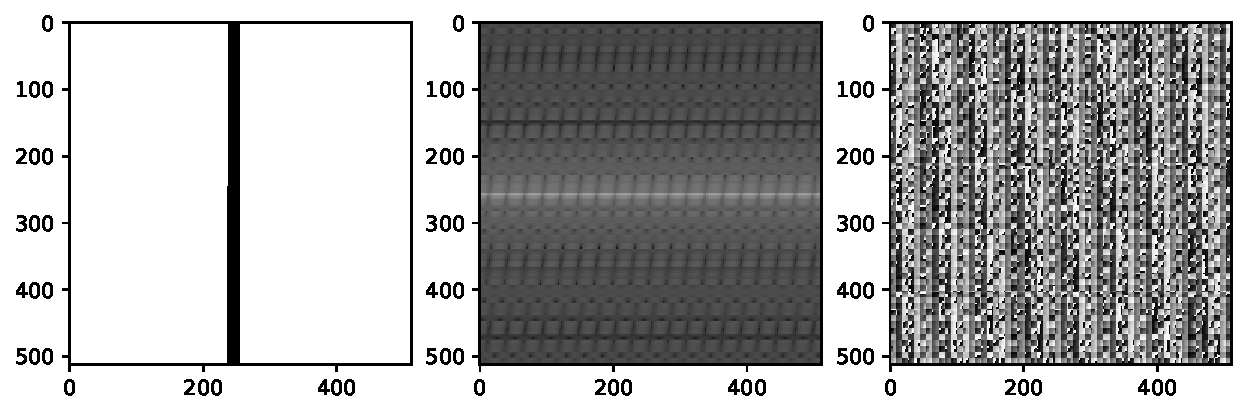
\includegraphics[height=6cm]{informe-imgs/ej3-e.pdf}
  \caption{\texttt{python practica4/fourier.py imgs-ej3/img-e.png}}
\end{figure}

\subsection{f) rotación de la linea a 45 grados}
\begin{figure}[H]
\centering
  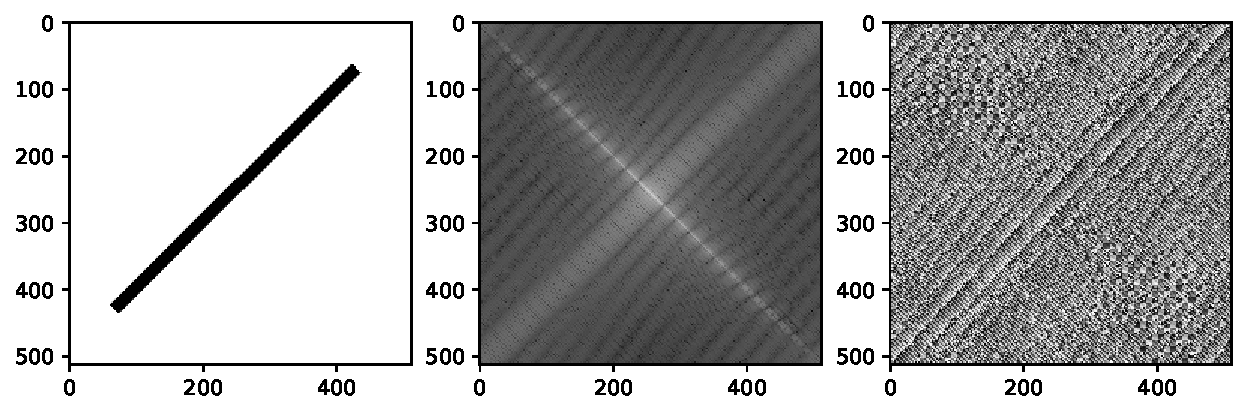
\includegraphics[height=6cm]{informe-imgs/ej3-f.pdf}
  \caption{\texttt{python practica4/fourier.py imgs-ej3/img-f.png}}
\end{figure}

\subsection{g) rotación de la linea a 90 grados}
\begin{figure}[H]
\centering
  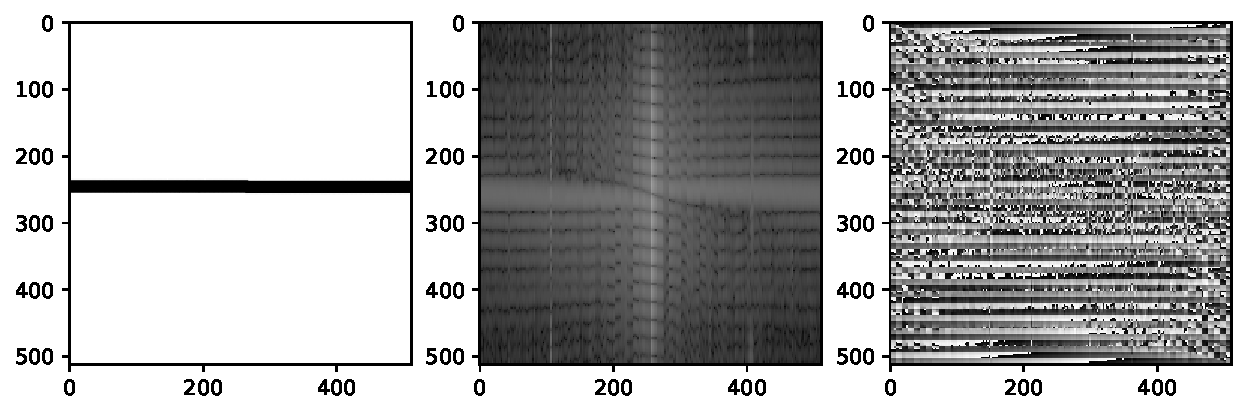
\includegraphics[height=6cm]{informe-imgs/ej3-g.pdf}
  \caption{\texttt{python practica4/fourier.py imgs-ej3/img-g.png}}
\end{figure}

\subsection{h) varias líneas vertical}
En estas imágenes sucede algo muy similar a lo que sucedía para las imágenes de una linea, pero aquí tenemos una señal
de período mas corto, luego el gráfico de fourier va a ser muy similar pero con período más corto
\begin{figure}[H]
\centering
  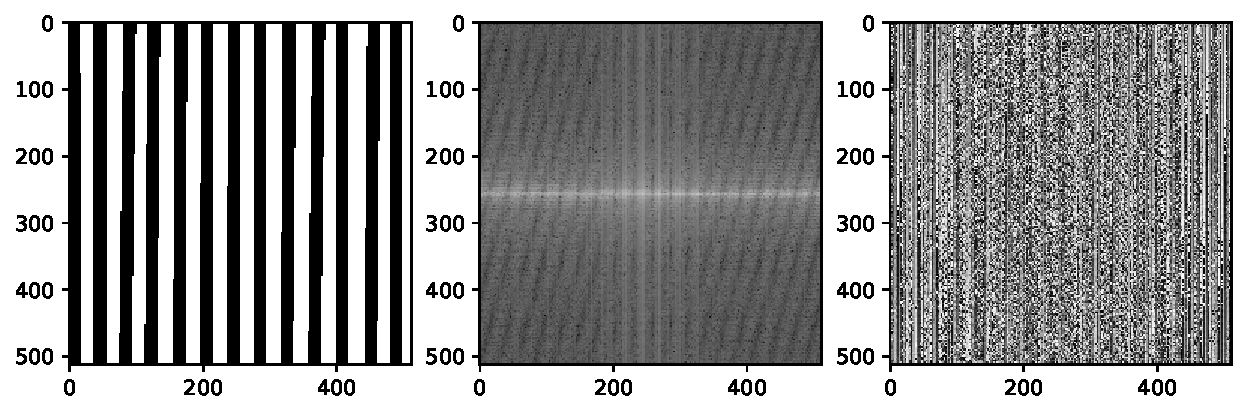
\includegraphics[height=6cm]{informe-imgs/ej3-h.pdf}
  \caption{\texttt{python practica4/fourier.py imgs-ej3/img-h.png}}
\end{figure}

\subsection{i) rotación de las líneas a 45 grados}
\begin{figure}[H]
\centering
  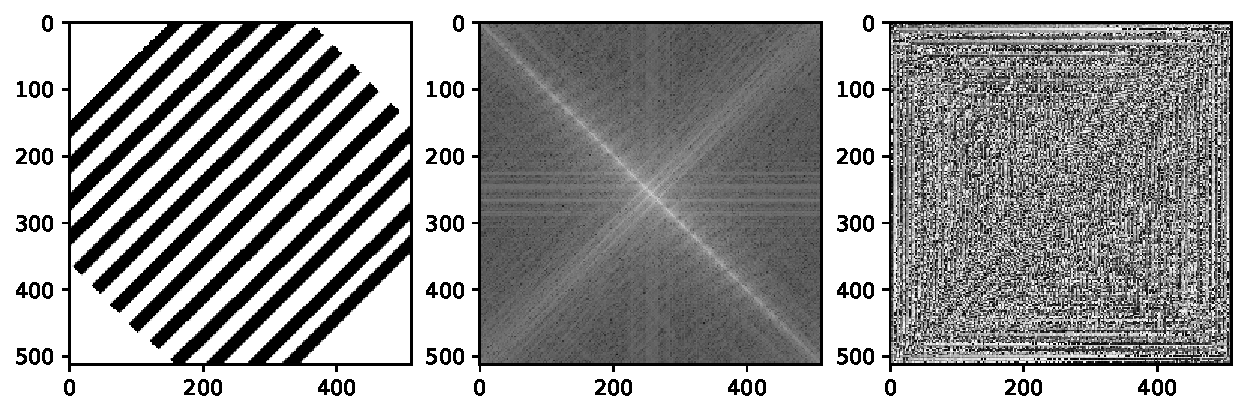
\includegraphics[height=6cm]{informe-imgs/ej3-i.pdf}
  \caption{\texttt{python practica4/fourier.py imgs-ej3/img-i.png}}
\end{figure}

\subsection{j) rotación de las líneas a 90 grados}
\begin{figure}[H]
\centering
  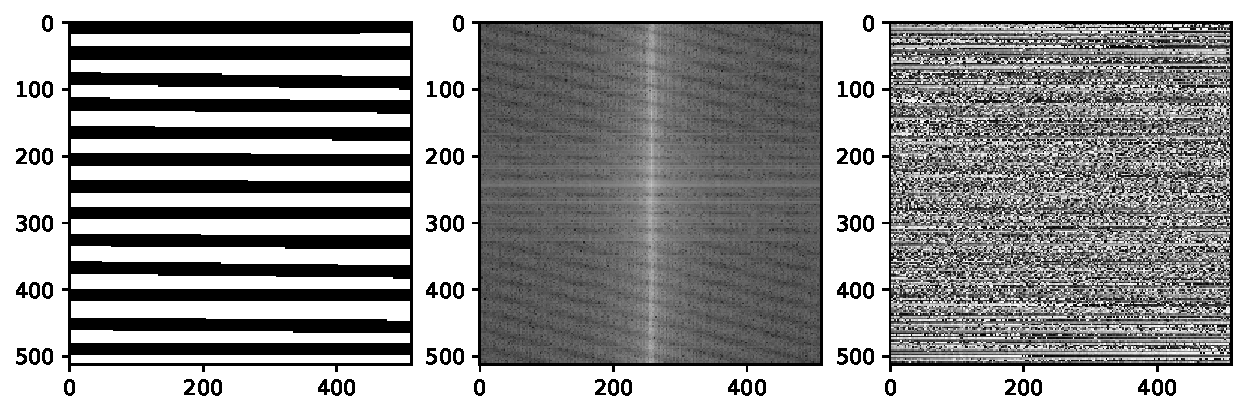
\includegraphics[height=6cm]{informe-imgs/ej3-j.pdf}
  \caption{\texttt{python practica4/fourier.py imgs-ej3/img-j.png}}
\end{figure}

\newpage
\section{Ejercicio 4}

Este ejercicio pide tomar el módulo y la fase de las transformadas de Fourier de dos imágenes y combinarlas.

Modo de uso
\begin{verbatim}
    python3 practica4/ej4.py <img1> <img2>
\end{verbatim}

\begin{figure}[H]
\centering
  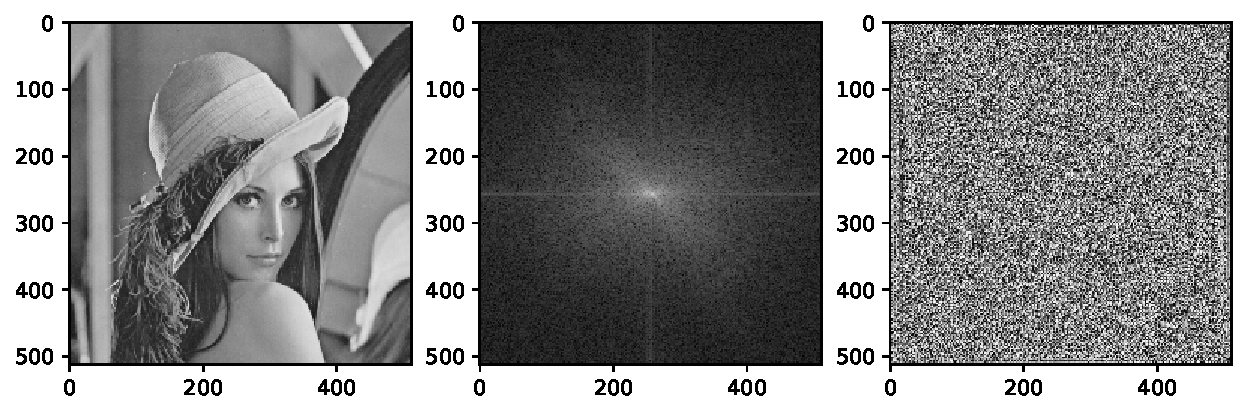
\includegraphics[height=6cm]{informe-imgs/ej4-lena.pdf}
  \caption{\texttt{python ej4.py lena.png ladrillos.png}}
\end{figure}

\begin{figure}[H]
\centering
  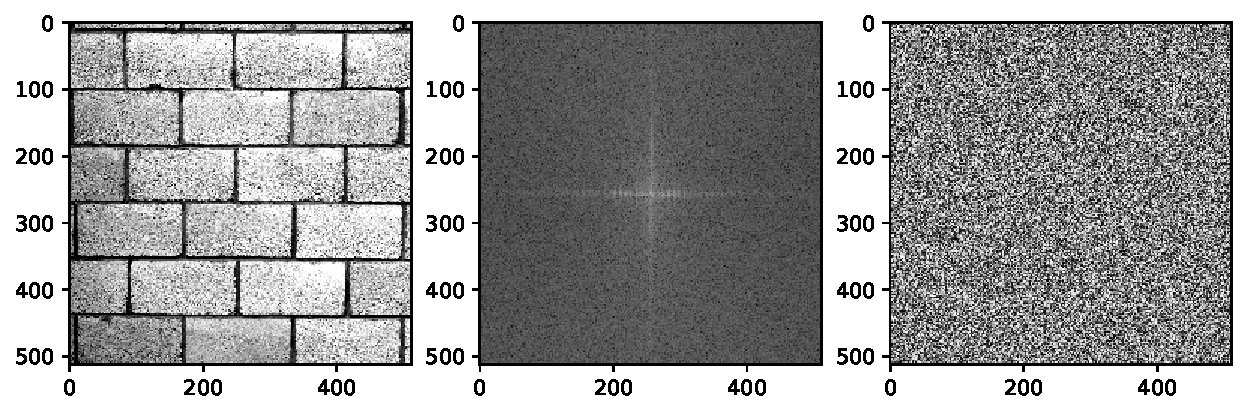
\includegraphics[height=6cm]{informe-imgs/ej4-ladrillos.pdf}
  \caption{\texttt{python ej4.py lena.png ladrillos.png}}
\end{figure}

Como se ve, la fase es muy importante para que se obtenga la figura que la transformada de fourier representa.

En la primera imagen, combinamos el módulo de lena con la fase de ladrillos, con lo cual vemos más notoriamente las
figuras de los ladrillos.
En la segunda, combinamos el módulo de la imagen de los ladrillos con la fase de la imagen de lena, con lo cual la
imagen de lena es mas visible en el resultado final.
\begin{figure}[H]
\centering
  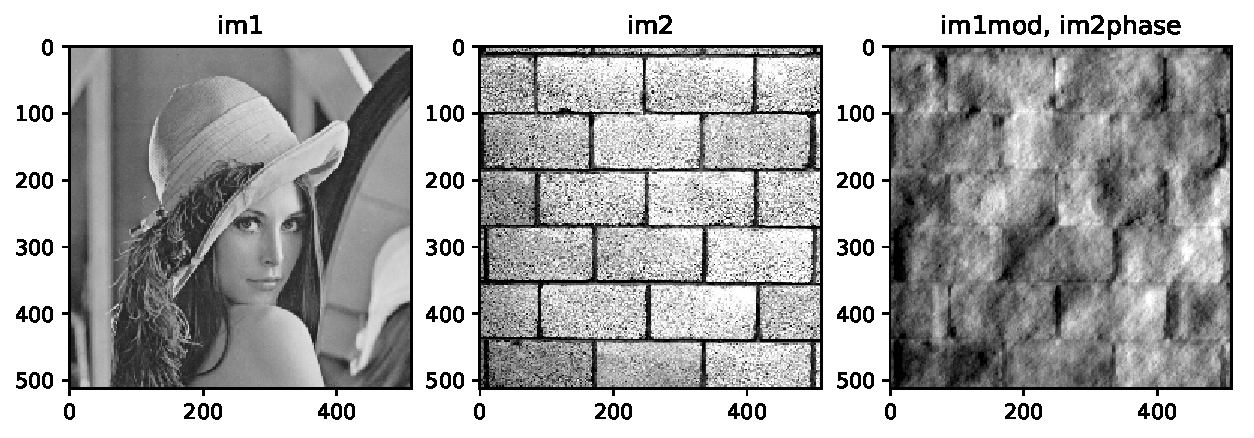
\includegraphics[height=6cm]{informe-imgs/ej4-a.pdf}
  \caption{\texttt{python ej4.py lena.png ladrillos.png}}
\end{figure}

\begin{figure}[H]
\centering
  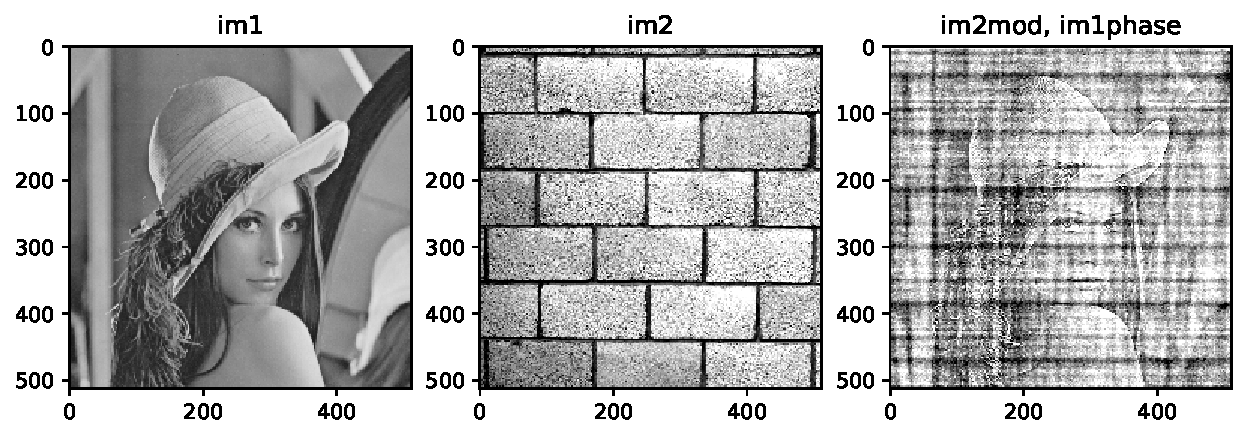
\includegraphics[height=6cm]{informe-imgs/ej4-b.pdf}
  \caption{\texttt{python ej4.py lena.png ladrillos.png}}
\end{figure}



\newpage
\section{Ejercicio 5}

En este ejercicio debemos combinar la imagen de Lena con la imagen de líneas, y luego recuperar a Lena usando la DFT.

Modo de uso
\begin{verbatim}
    python3 practica4/ej5.py <img1> <img2>
\end{verbatim}


\begin{figure}[H]
\centering
  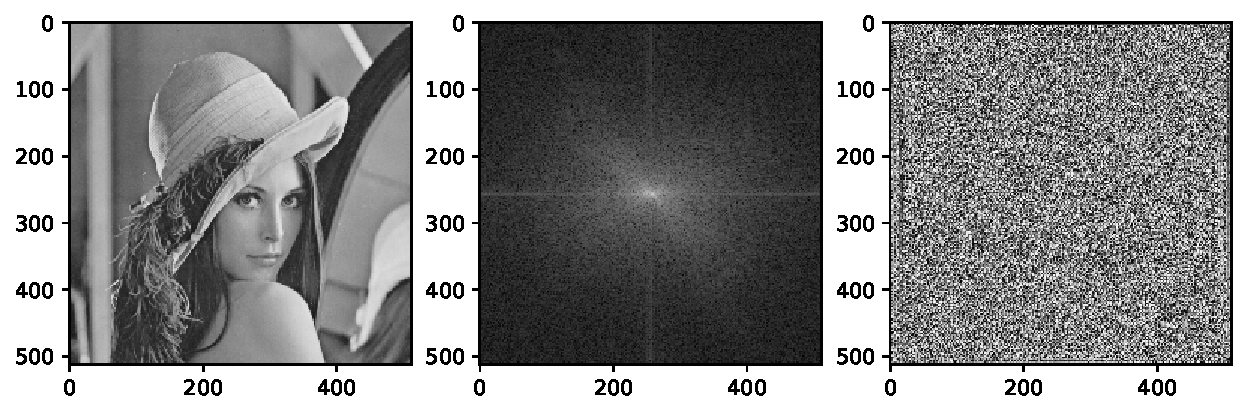
\includegraphics[height=6cm]{informe-imgs/ej5-lena.pdf}
  \caption{\texttt{python ej5.py lena.png lineas.png}. Lena.}
\end{figure}

\begin{figure}[H]
\centering
  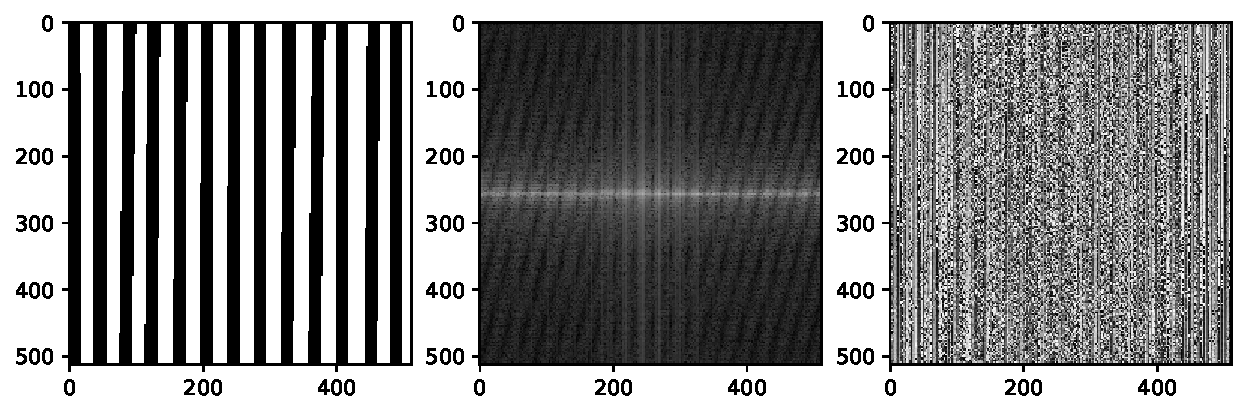
\includegraphics[height=6cm]{informe-imgs/ej5-lineas.pdf}
  \caption{\texttt{python ej5.py lena.png lineas.png}. Líneas.}
\end{figure}

\begin{figure}[H]
\centering
  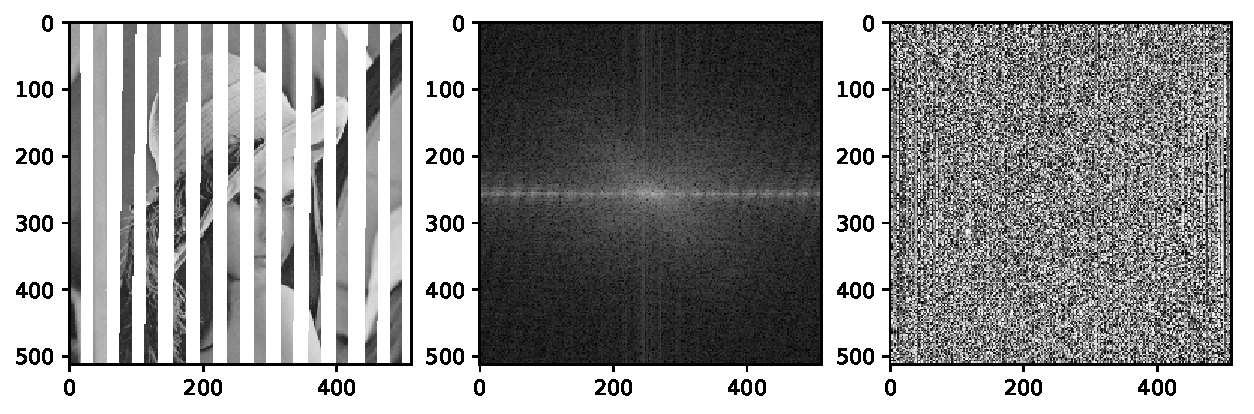
\includegraphics[height=6cm]{informe-imgs/ej5-suma.pdf}
  \caption{\texttt{python ej5.py lena.png lineas.png}. Suma de lena y líneas.}
\end{figure}

Allí tenemos la suma de las imágenes.

Para recuperar la imagen original intenté varias cosas. Basándome en el ejercicio anterior me enfoque en la fase de la
imagen, pero eso no llegó a ningun resultado positivo.

Sin embargo, tomar el DFT de la suma y modificar el módulo, restándole el de las líneas y sumándole el de lena mejora la
imagen bastante, y el resultado es el que está a continuación.

\begin{figure}[H]
\centering
  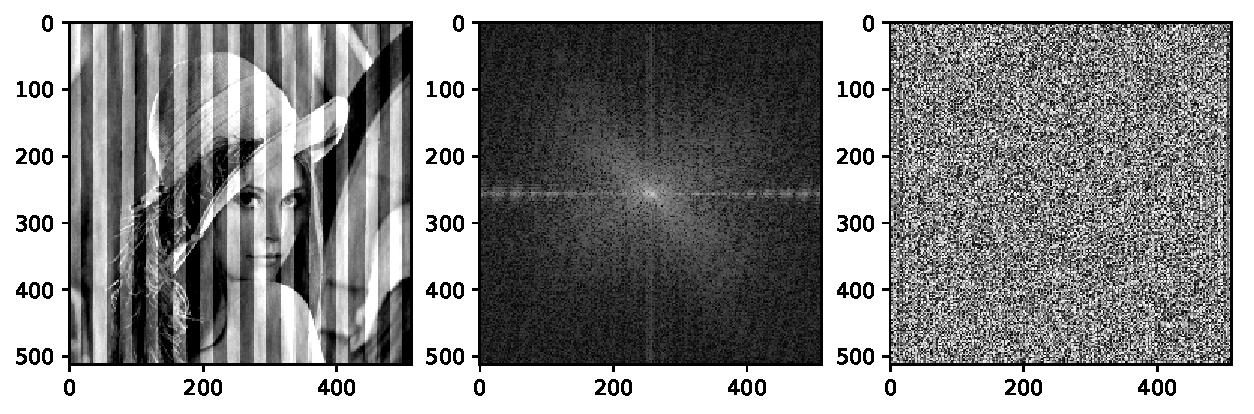
\includegraphics[height=6cm]{informe-imgs/ej5-res.pdf}
  \caption{\texttt{python ej5.py lena.png lineas.png}. Luego de sacar las líneas usando la DFT.}
\end{figure}



\newpage
\section{Ejercicio 6}
Fue hecho en la entrega escrita de la práctica 4.


\end{document}
